\section{Large Language Models}
\label{sec:llm}

Large Language Models (LLMs) represent a class of artificial intelligence systems trained on vast corpora of text data to understand and generate human language \cite{brown2020language}. These models have demonstrated remarkable capabilities in natural language understanding, reasoning, and generation, enabling a wide range of applications from conversational assistants to code synthesis. This section examines the fundamental concepts underlying LLMs and their relevance to the development of intelligent agents.

\subsection{Transformer Architecture}

Modern LLMs are built upon the Transformer architecture, introduced by Vaswani et al. in 2017. The Transformer revolutionized natural language processing by replacing recurrent neural network architectures with self-attention mechanisms, enabling efficient parallel processing of sequential data and capturing long-range dependencies in text.

The self-attention mechanism allows each token in a sequence to attend to all other tokens, computing relevance weights that determine how much information to gather from each position. This is expressed mathematically as:

\begin{equation}
    \text{Attention}(Q, K, V) = \text{softmax}\left(\frac{QK^T}{\sqrt{d_k}}\right)V
\end{equation}

where $Q$, $K$, and $V$ represent query, key, and value matrices derived from the input, and $d_k$ is the dimension of the key vectors. The scaling factor $\sqrt{d_k}$ prevents the softmax function from entering regions of extremely small gradients.

% Placeholder: Transformer architecture diagram
\begin{figure}[H]
    \centering
    % \fbox{\parbox{0.8\textwidth}{\centering \textit{[Placeholder: Diagram of the Transformer architecture showing encoder-decoder structure with attention layers]}}}
    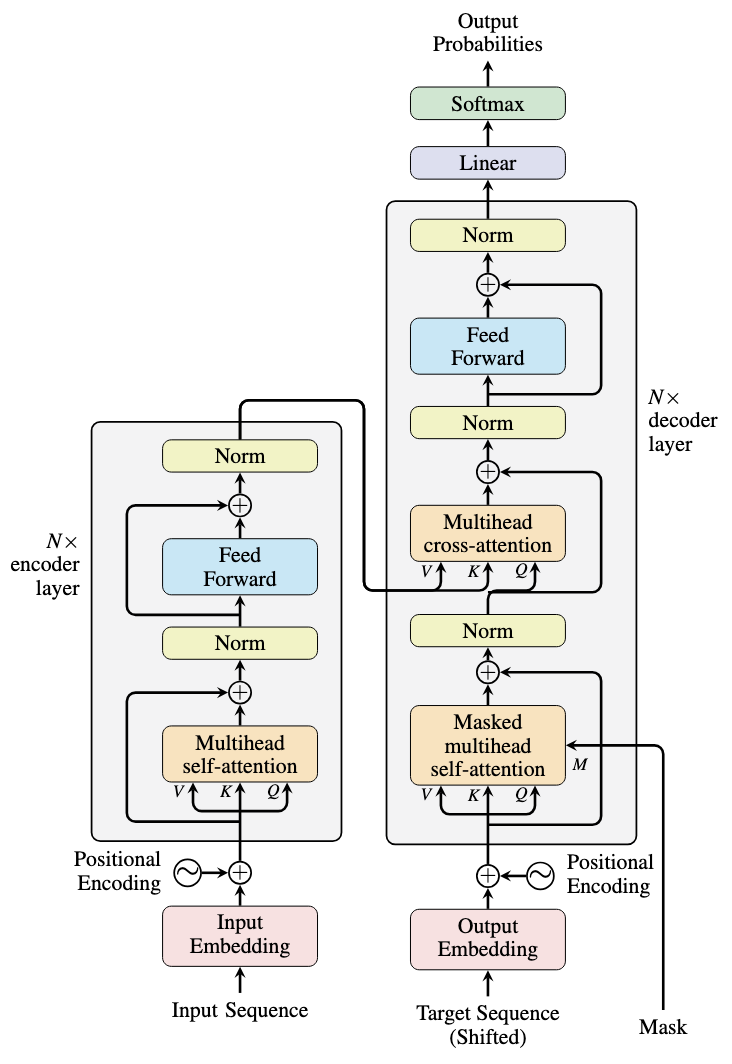
\includegraphics[width=0.5\textwidth]{images/transformer_architecture.png}
    \caption{Transformer Architecture Overview}
    \label{fig:transformer}
\end{figure}

Transformers typically employ multi-head attention, where multiple attention computations are performed in parallel with different learned projections. This enables the model to capture different types of relationships and patterns simultaneously:

\begin{equation}
    \text{MultiHead}(Q, K, V) = \text{Concat}(\text{head}_1, ..., \text{head}_h)W^O
\end{equation}

The architecture includes layer normalization, residual connections, and position-wise feed-forward networks that contribute to training stability and model expressiveness.

\subsection{Autoregressive Language Modeling}

LLMs are typically trained using autoregressive language modeling, where the model learns to predict the next token in a sequence given all preceding tokens. This training objective can be formalized as maximizing the log-likelihood:

\begin{equation}
    \mathcal{L}(\theta) = \sum_{i=1}^{n} \log P(x_i | x_1, x_2, ..., x_{i-1}; \theta)
\end{equation}

where $\theta$ represents the model parameters and $x_1, ..., x_n$ is the training sequence.

During inference, the model generates text by sampling or selecting tokens autoregressively, where each generated token becomes part of the context for generating subsequent tokens. Various decoding strategies exist, including:
\begin{itemize}
    \item \textbf{Greedy decoding}: Always selecting the highest-probability token
    \item \textbf{Beam search}: Maintaining multiple candidate sequences simultaneously
    \item \textbf{Sampling}: Probabilistically selecting tokens based on the predicted distribution
    \item \textbf{Top-k/Top-p sampling}: Restricting sampling to the most likely candidates
\end{itemize}

\subsection{Instruction Tuning and Alignment}

While base language models are trained purely on next-token prediction, they require additional training to become useful assistants. Instruction tuning fine-tunes models on datasets of instructions paired with desired responses, enabling the model to follow user directives effectively.

Reinforcement Learning from Human Feedback (RLHF) further aligns models with human preferences \cite{bai2022constitutional}. This process involves:
\begin{enumerate}
    \item Training a reward model on human preference data
    \item Using the reward model to provide training signal
    \item Optimizing the language model policy using reinforcement learning algorithms
\end{enumerate}

The alignment process helps models produce outputs that are helpful, harmless, and honest—critical properties for deployment in real-world applications.

\subsection{Emergent Capabilities}

As LLMs scale in parameters and training data, they exhibit emergent capabilities not explicitly trained for. These include:

\textbf{In-context learning}: The ability to learn new tasks from examples provided in the prompt, without parameter updates. By presenting a few demonstrations of the desired input-output mapping, the model can generalize to new inputs.

\textbf{Chain-of-thought reasoning}: When prompted appropriately, LLMs can generate intermediate reasoning steps that improve performance on complex problems. This capability is particularly important for multi-step tasks requiring logical deduction.

\textbf{Tool use}: Models can learn to interact with external tools and APIs by generating appropriate function calls or structured outputs. This capability enables LLMs to access real-time information, perform calculations, and interact with external systems.

\subsection{Function Calling and Structured Output}

Modern LLMs support function calling, where the model can output structured requests to invoke external tools. Given a set of available functions with specified parameter schemas, the model determines when to call functions and how to construct appropriate arguments.

The function calling paradigm follows this pattern:
\begin{enumerate}
    \item The system prompt defines available functions with their descriptions and parameter schemas
    \item The model receives a user query and determines if function calls are needed
    \item The model outputs structured function call requests with appropriate arguments
    \item The application executes the function and returns results to the model
    \item The model incorporates results and continues generation
\end{enumerate}

This capability is fundamental to building LLM-based agents, as it provides the mechanism by which language models can take actions in the world rather than merely generating text responses.
